\subsection*{Venneliste}
Venneliste inddeles i to boundaryklasser og en dertilhørende controlklasse, som fremgår af \autoref{fig:MVCVenneliste}. 

\begin{figure} [H]
\centering
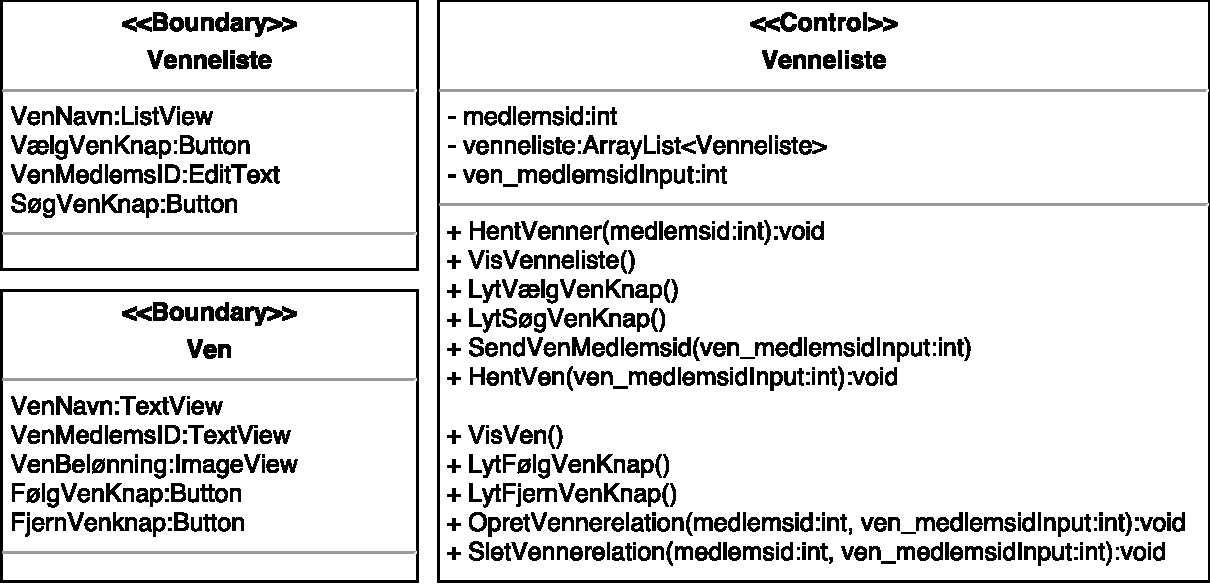
\includegraphics[width=0.8\textwidth]{figures/MVC/MVCVenneliste}
\caption{Designklasser for venneliste. Til venstre ses boundary for Venneliste og Ven, hvor der til højre ses tilhørende controller.}
\label{fig:MVCVenneliste}
\end{figure}

\noindent
I grænsefladen \textit{Venneliste} findes tekstfelter, af typen TextView, med fornavn og efternavn på de brugere, der følges. Hver bruger, der vises af den givne grænseflade, kan tilgås ved at trykke på brugeren. Derudover er der i denne grænseflade et søgefelt, af typen EditText, med en tilhørende SøgKnap, af typen Button, som muliggør, at brugeren kan søge på andre brugere med deres medlemsID. 
Når en bruger tilgås, enten via vennelisten eller ved at søge på en bruger, vises grænsefladen for den pågældende ven. Hertil vises  tekstfelter, af typen TextView, med brugerens medlemsID, fornavn, efternavn samt vedkommendes belønninger. Hvis brugeren ikke følges, er der her opstillet en FølgKnap.
Den tilhørende controller har metoderne Vis, Hent, Lyt, Valider og Opret. 
Ud fra de nævnte designklasser er udarbejdet et sekvensdiagram, der fremgår af \autoref{fig:SEKVenneliste}.

\begin{figure} [H]
\centering
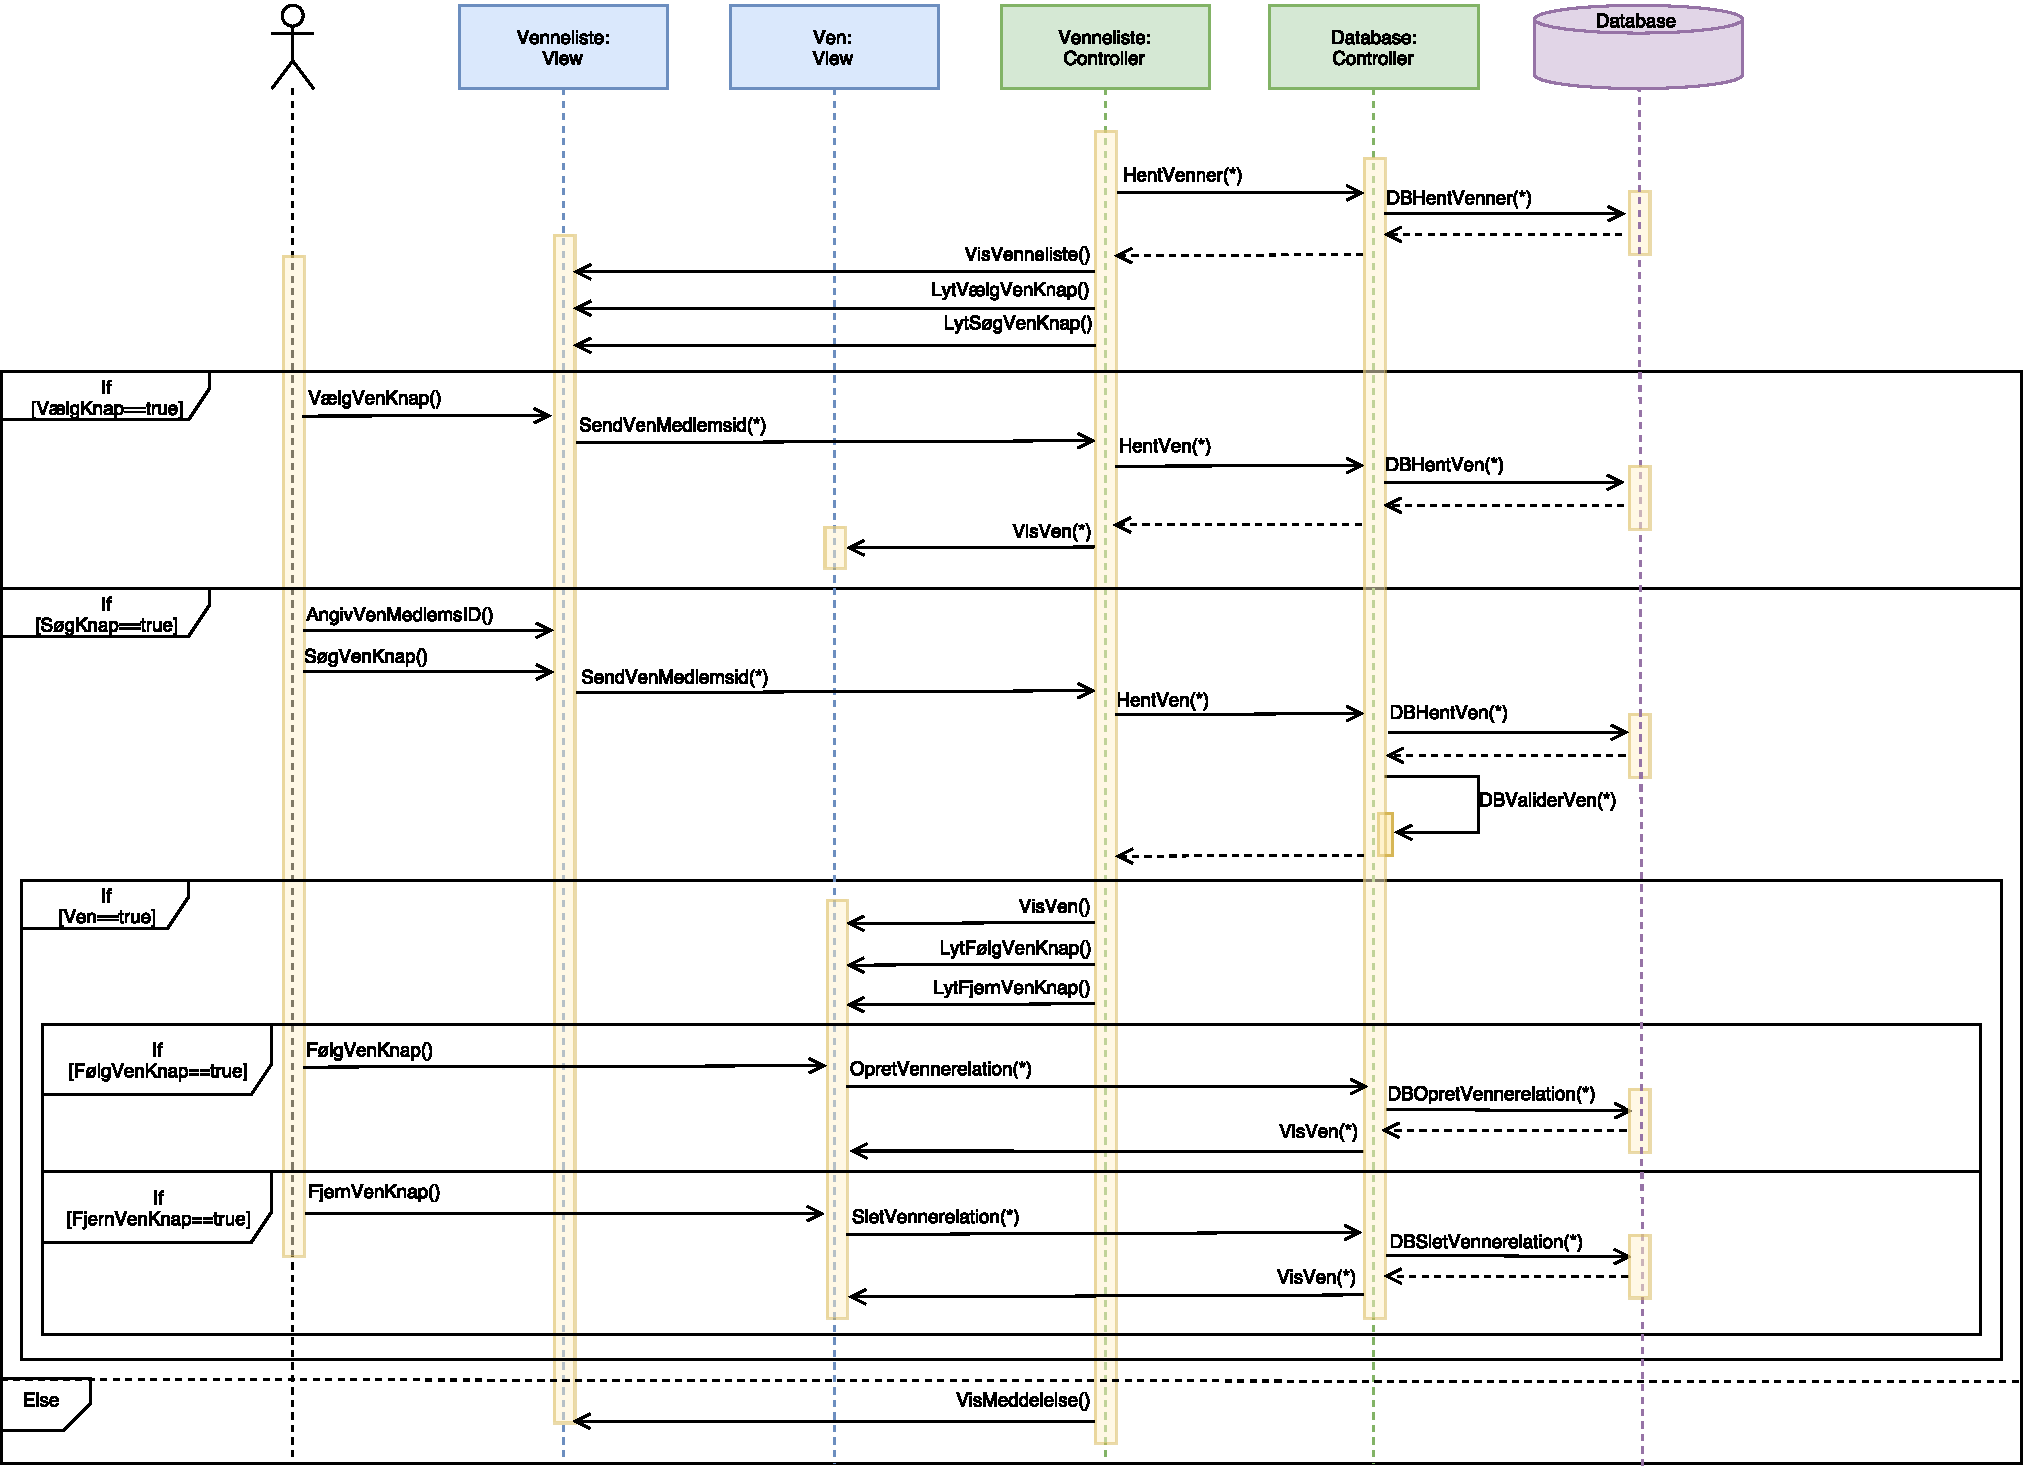
\includegraphics[width=1.55\textwidth, angle=90]{figures/Sek/SEKVenneliste}
\caption{Sekvensdiagram for venneliste.}
\label{fig:SEKVenneliste}
\end{figure}

\noindent
Controlleren henter brugerens venneliste fra vennelistemodellen, hvorefter grænsefladen for venneliste vises. Dertil lytter controlleren på VenKnap samt SøgKnap. Vælger brugeren at tilgå en ven fra vennelisten, vises grænsefladen for den valgte ven. Vælger brugeren derimod at søge efter en anden bruger, hentes det indskrevne medlemsID, således den søgte bruger kan findes i databasen, hvortil den valideres. Såfremt brugeren findes i databasen, vises VenOplysninger, hvorimod en grænseflade for fejlmeddelelse vises, hvis brugeren ikke findes. Brugeren skal herved benytte OKKnap på grænsefladen for at bekræfte, at fejlen er set, hvorefter systemet returneres til brugerens venneliste.
Grænsefladen for den søgte ven tillader ligeledes muligheden for at følge brugeren, hvis vedkommende ikke følges. Ønskes det at følge brugeren, oprettes en vennerelation i vennelistemodellen. 



%Venneliste inddeles i en grænseflade og dertilhørende controller, som det fremgår af \autoref{fig:MVCVenneliste}. 

%\begin{figure} [H]
%\centering
%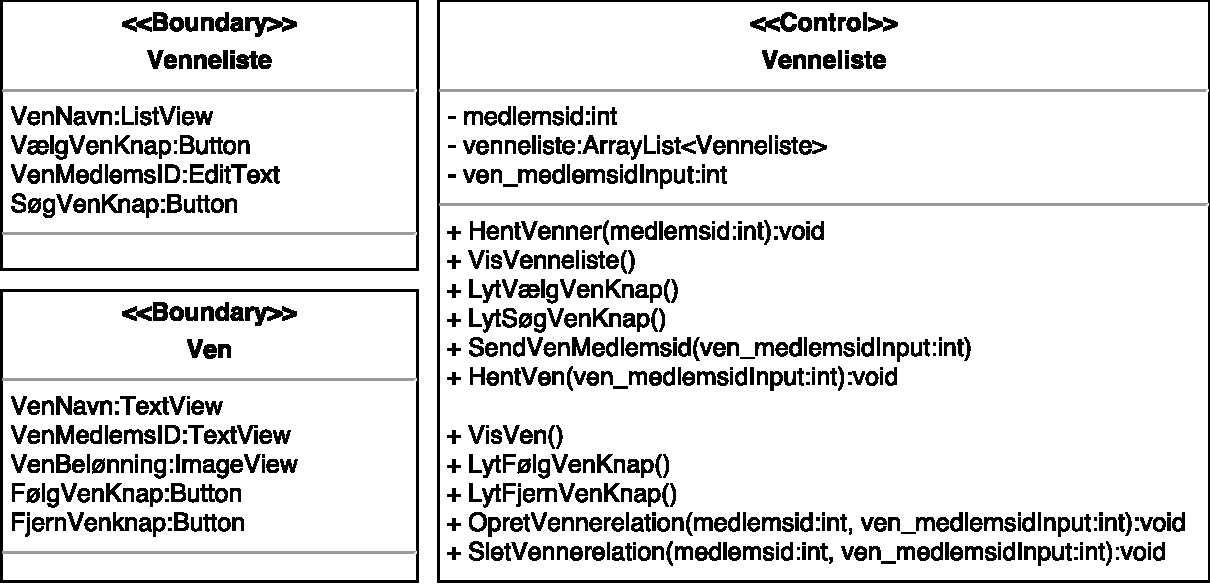
\includegraphics[width=0.8\textwidth]{figures/MVC/MVCVenneliste}
%\caption{Designklasser for venneliste.}
%\label{fig:MVCVenneliste}
%\end{figure}

%\noindent
%\textit{VennelisteGrænsefladen} indeholder tekstfelter for fornavn og efternavn på de brugere de følger. Derudover er der opstillet tekstfelt for medlemsID, hvor brugeren kan angive medlemsID'et på en bruger de ønsker at følge. Dertil er der opstillet en tilhørende søge knap, af typen button, der ved tryk indikere at brugeren har angivet medlemsID på brugeren den ønsker at følge. Derudover har brugeren mulighed for at vælge en bruger eller gå tilbage via en vælg eller tilbage  knap, der også er af typen button. 


%Der er til \textit{VennelisteGrænsefladen} opstillet en \textit{VennelisteController}, der har til formål at vise en oversigt over vennelisten når grænsefladen for vennelisten tilgås. Brugeren har via vælg knappen mulighed for at tilgå en bruger den følger
%Controlleren lytter på om brugeren trykker på vælg knappen eller søg knappen. Vælg knappen giver brugeren mulighed for at tilgå enkelt bruger ud fra vennelisten. Trykker brugeren på søg knappen kontrollere controlleren om det angivne medlemsID findes i databasen, herefter kan brugeren trykke på vælg. Trykkes der på en af vælg knapperne, enten i vennelisten eller efter søgning på medlemsID vises \textit{VenGrænsefladen}, som fremgår af \autoref{MVCVen}. Controlleren lytter på tilbage knappen, hvis denne trykkes på vises forrige grænseflade. 


%\subsubsection*{Ven}
%Ven inddeles i en grænseflade og tilhørende controller, som det fremgår af \autoref{fig:MVCVen}.

%\begin{figure} [H]
%\centering
%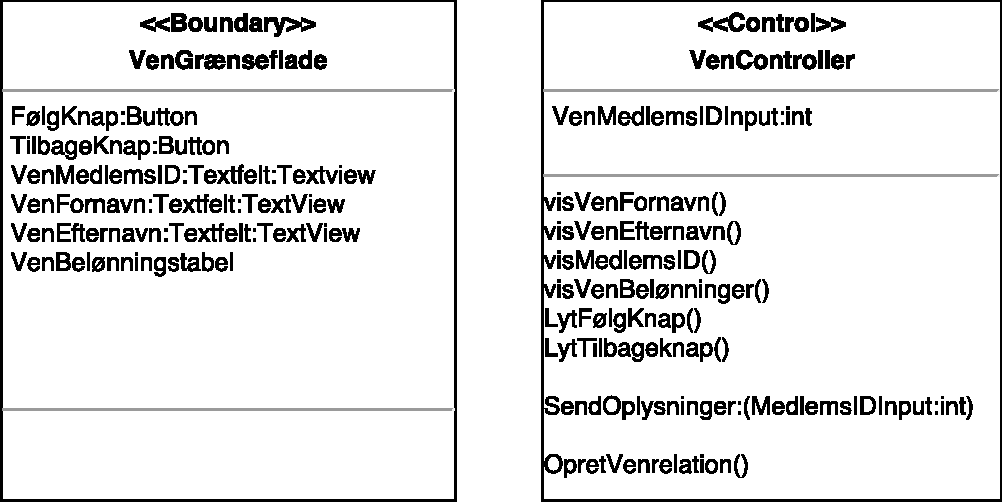
\includegraphics[width=0.8\textwidth]{figures/MVC/MVCVen}
%\caption{Designklasser for ven.}
%\label{fig:MVCVen}
%\end{figure}

%\noindent
%I \textit{VenGrænseflade} vises tekstfelter for valgt bruger, herunder MedlemsID, fornavn og efternavn. Dertil er der opstillet en følg knap og en tilbage knap af typen button. Følg knap er kun tilgængelig, hvis brugeren ikke følger den valgte ven. Derudover vises en tabel med den valgte brugers belønninger.


%Til \textit{VenGrænsefladen} er der opstillet en \textit{VenController}, som har til formål vise brugeroplysninger, herunder MedlemsID, fornavn og efternavn samt belønningstabel for den valgte bruger. Controlleren lytter på om brugeren trykker på følg knappen, hvis brugeren ikke allerede følger eller trykker på tilbage knappen. Trykkes der på følg knappen sendes MedlemsID'et på den bruger der ønskes at følges til databasen, hvorefter vennerelation gemmes i denne. Vælger brugeren at trykke på tilbage knappen vises den forrige grænseflade.   